% Options for packages loaded elsewhere
\PassOptionsToPackage{unicode}{hyperref}
\PassOptionsToPackage{hyphens}{url}
%
\documentclass[
  oneside,
  open=any]{scrbook}

\usepackage{amsmath,amssymb}
\usepackage{lmodern}
\usepackage{iftex}
\ifPDFTeX
  \usepackage[T1]{fontenc}
  \usepackage[utf8]{inputenc}
  \usepackage{textcomp} % provide euro and other symbols
\else % if luatex or xetex
  \usepackage{unicode-math}
  \defaultfontfeatures{Scale=MatchLowercase}
  \defaultfontfeatures[\rmfamily]{Ligatures=TeX,Scale=1}
\fi
% Use upquote if available, for straight quotes in verbatim environments
\IfFileExists{upquote.sty}{\usepackage{upquote}}{}
\IfFileExists{microtype.sty}{% use microtype if available
  \usepackage[]{microtype}
  \UseMicrotypeSet[protrusion]{basicmath} % disable protrusion for tt fonts
}{}
\makeatletter
\@ifundefined{KOMAClassName}{% if non-KOMA class
  \IfFileExists{parskip.sty}{%
    \usepackage{parskip}
  }{% else
    \setlength{\parindent}{0pt}
    \setlength{\parskip}{6pt plus 2pt minus 1pt}}
}{% if KOMA class
  \KOMAoptions{parskip=half}}
\makeatother
\usepackage{xcolor}
\setlength{\emergencystretch}{3em} % prevent overfull lines
\setcounter{secnumdepth}{5}
% Make \paragraph and \subparagraph free-standing
\ifx\paragraph\undefined\else
  \let\oldparagraph\paragraph
  \renewcommand{\paragraph}[1]{\oldparagraph{#1}\mbox{}}
\fi
\ifx\subparagraph\undefined\else
  \let\oldsubparagraph\subparagraph
  \renewcommand{\subparagraph}[1]{\oldsubparagraph{#1}\mbox{}}
\fi

\providecommand{\tightlist}{%
  \setlength{\itemsep}{0pt}\setlength{\parskip}{0pt}}\usepackage{longtable,booktabs,array}
\usepackage{calc} % for calculating minipage widths
% Correct order of tables after \paragraph or \subparagraph
\usepackage{etoolbox}
\makeatletter
\patchcmd\longtable{\par}{\if@noskipsec\mbox{}\fi\par}{}{}
\makeatother
% Allow footnotes in longtable head/foot
\IfFileExists{footnotehyper.sty}{\usepackage{footnotehyper}}{\usepackage{footnote}}
\makesavenoteenv{longtable}
\usepackage{graphicx}
\makeatletter
\def\maxwidth{\ifdim\Gin@nat@width>\linewidth\linewidth\else\Gin@nat@width\fi}
\def\maxheight{\ifdim\Gin@nat@height>\textheight\textheight\else\Gin@nat@height\fi}
\makeatother
% Scale images if necessary, so that they will not overflow the page
% margins by default, and it is still possible to overwrite the defaults
% using explicit options in \includegraphics[width, height, ...]{}
\setkeys{Gin}{width=\maxwidth,height=\maxheight,keepaspectratio}
% Set default figure placement to htbp
\makeatletter
\def\fps@figure{htbp}
\makeatother
\newlength{\cslhangindent}
\setlength{\cslhangindent}{1.5em}
\newlength{\csllabelwidth}
\setlength{\csllabelwidth}{3em}
\newlength{\cslentryspacingunit} % times entry-spacing
\setlength{\cslentryspacingunit}{\parskip}
\newenvironment{CSLReferences}[2] % #1 hanging-ident, #2 entry spacing
 {% don't indent paragraphs
  \setlength{\parindent}{0pt}
  % turn on hanging indent if param 1 is 1
  \ifodd #1
  \let\oldpar\par
  \def\par{\hangindent=\cslhangindent\oldpar}
  \fi
  % set entry spacing
  \setlength{\parskip}{#2\cslentryspacingunit}
 }%
 {}
\usepackage{calc}
\newcommand{\CSLBlock}[1]{#1\hfill\break}
\newcommand{\CSLLeftMargin}[1]{\parbox[t]{\csllabelwidth}{#1}}
\newcommand{\CSLRightInline}[1]{\parbox[t]{\linewidth - \csllabelwidth}{#1}\break}
\newcommand{\CSLIndent}[1]{\hspace{\cslhangindent}#1}

\makeatletter
\makeatother
\makeatletter
\makeatother
\makeatletter
\@ifpackageloaded{caption}{}{\usepackage{caption}}
\AtBeginDocument{%
\ifdefined\contentsname
  \renewcommand*\contentsname{Table of contents}
\else
  \newcommand\contentsname{Table of contents}
\fi
\ifdefined\listfigurename
  \renewcommand*\listfigurename{List of Figures}
\else
  \newcommand\listfigurename{List of Figures}
\fi
\ifdefined\listtablename
  \renewcommand*\listtablename{List of Tables}
\else
  \newcommand\listtablename{List of Tables}
\fi
\ifdefined\figurename
  \renewcommand*\figurename{Figure}
\else
  \newcommand\figurename{Figure}
\fi
\ifdefined\tablename
  \renewcommand*\tablename{Table}
\else
  \newcommand\tablename{Table}
\fi
}
\@ifpackageloaded{float}{}{\usepackage{float}}
\floatstyle{ruled}
\@ifundefined{c@chapter}{\newfloat{codelisting}{h}{lop}}{\newfloat{codelisting}{h}{lop}[chapter]}
\floatname{codelisting}{Listing}
\newcommand*\listoflistings{\listof{codelisting}{List of Listings}}
\makeatother
\makeatletter
\@ifpackageloaded{caption}{}{\usepackage{caption}}
\@ifpackageloaded{subcaption}{}{\usepackage{subcaption}}
\makeatother
\makeatletter
\@ifpackageloaded{tcolorbox}{}{\usepackage[many]{tcolorbox}}
\makeatother
\makeatletter
\@ifundefined{shadecolor}{\definecolor{shadecolor}{rgb}{.97, .97, .97}}
\makeatother
\makeatletter
\makeatother

\usepackage{hyphenat}
\usepackage{ifthen}
\usepackage{calc}
\usepackage{calculator}



\usepackage{graphicx}
\usepackage{geometry}
\usepackage{afterpage}
\usepackage{tikz}
\usetikzlibrary{calc}
\usetikzlibrary{fadings}
\usepackage[pagecolor=none]{pagecolor}


\usepackage{fontspec}
\newfontfamily{\coverpagetitlefont}{QTHelvet-BoldOutline.otf}
\usepackage{fontspec}
\newfontfamily{\coverpageauthorfont}{Palatino}

% Set the titlepage font families
\usepackage{fontspec}
\newfontfamily{\titlepagefont}{QTDublinIrish.otf}

\newcommand{\titlepagetitlefont}{}

\newcommand{\titlepageauthorfont}{}

\newcommand{\titlepageaffiliationfont}{}

\usepackage{fontspec}
\newfontfamily{\titlepagefooterfont}{Palatino}

\newcommand{\titlepageheaderfont}{}
\ifLuaTeX
  \usepackage{selnolig}  % disable illegal ligatures
\fi
\IfFileExists{bookmark.sty}{\usepackage{bookmark}}{\usepackage{hyperref}}
\IfFileExists{xurl.sty}{\usepackage{xurl}}{} % add URL line breaks if available
\urlstyle{same} % disable monospaced font for URLs
\hypersetup{
  pdftitle={A Sample Title - The SocioEconomic Aspects of Stock Assessments},
  pdfauthor={Jane Doe; Eva Nováková; Matti Meikäläinen; Ashok Kumar},
  hidelinks,
  pdfcreator={LaTeX via pandoc}}

\title{A Sample Title - The SocioEconomic Aspects of Stock Assessments}
\usepackage{etoolbox}
\makeatletter
\providecommand{\subtitle}[1]{% add subtitle to \maketitle
  \apptocmd{\@title}{\par {\large #1 \par}}{}{}
}
\makeatother
\subtitle{with non-English diacritics in the author names. see
documentation.}
\author{Jane Doe \and Eva Nováková \and Matti Meikäläinen \and Ashok
Kumar}
\date{}

\begin{document}
  \begin{frontmatter}

\begin{titlepage}
% This is a combination of Pandoc templating and LaTeX
% Pandoc templating https://pandoc.org/MANUAL.html#templates
% See the README for help

\thispagestyle{empty}

\newgeometry{top=-100in}

% Page color

\begin{tikzpicture}[remember picture, overlay, inner sep=0pt, outer sep=0pt]

\tikzfading[name=fadeout, inner color=transparent!0,outer color=transparent!100]
\tikzfading[name=fadein, inner color=transparent!100,outer color=transparent!0]
\node[%
%
anchor=south west%
%
, opacity=0.5%
] at %
($(current page.south west)+(%
0cm,%
0cm%
)$) {
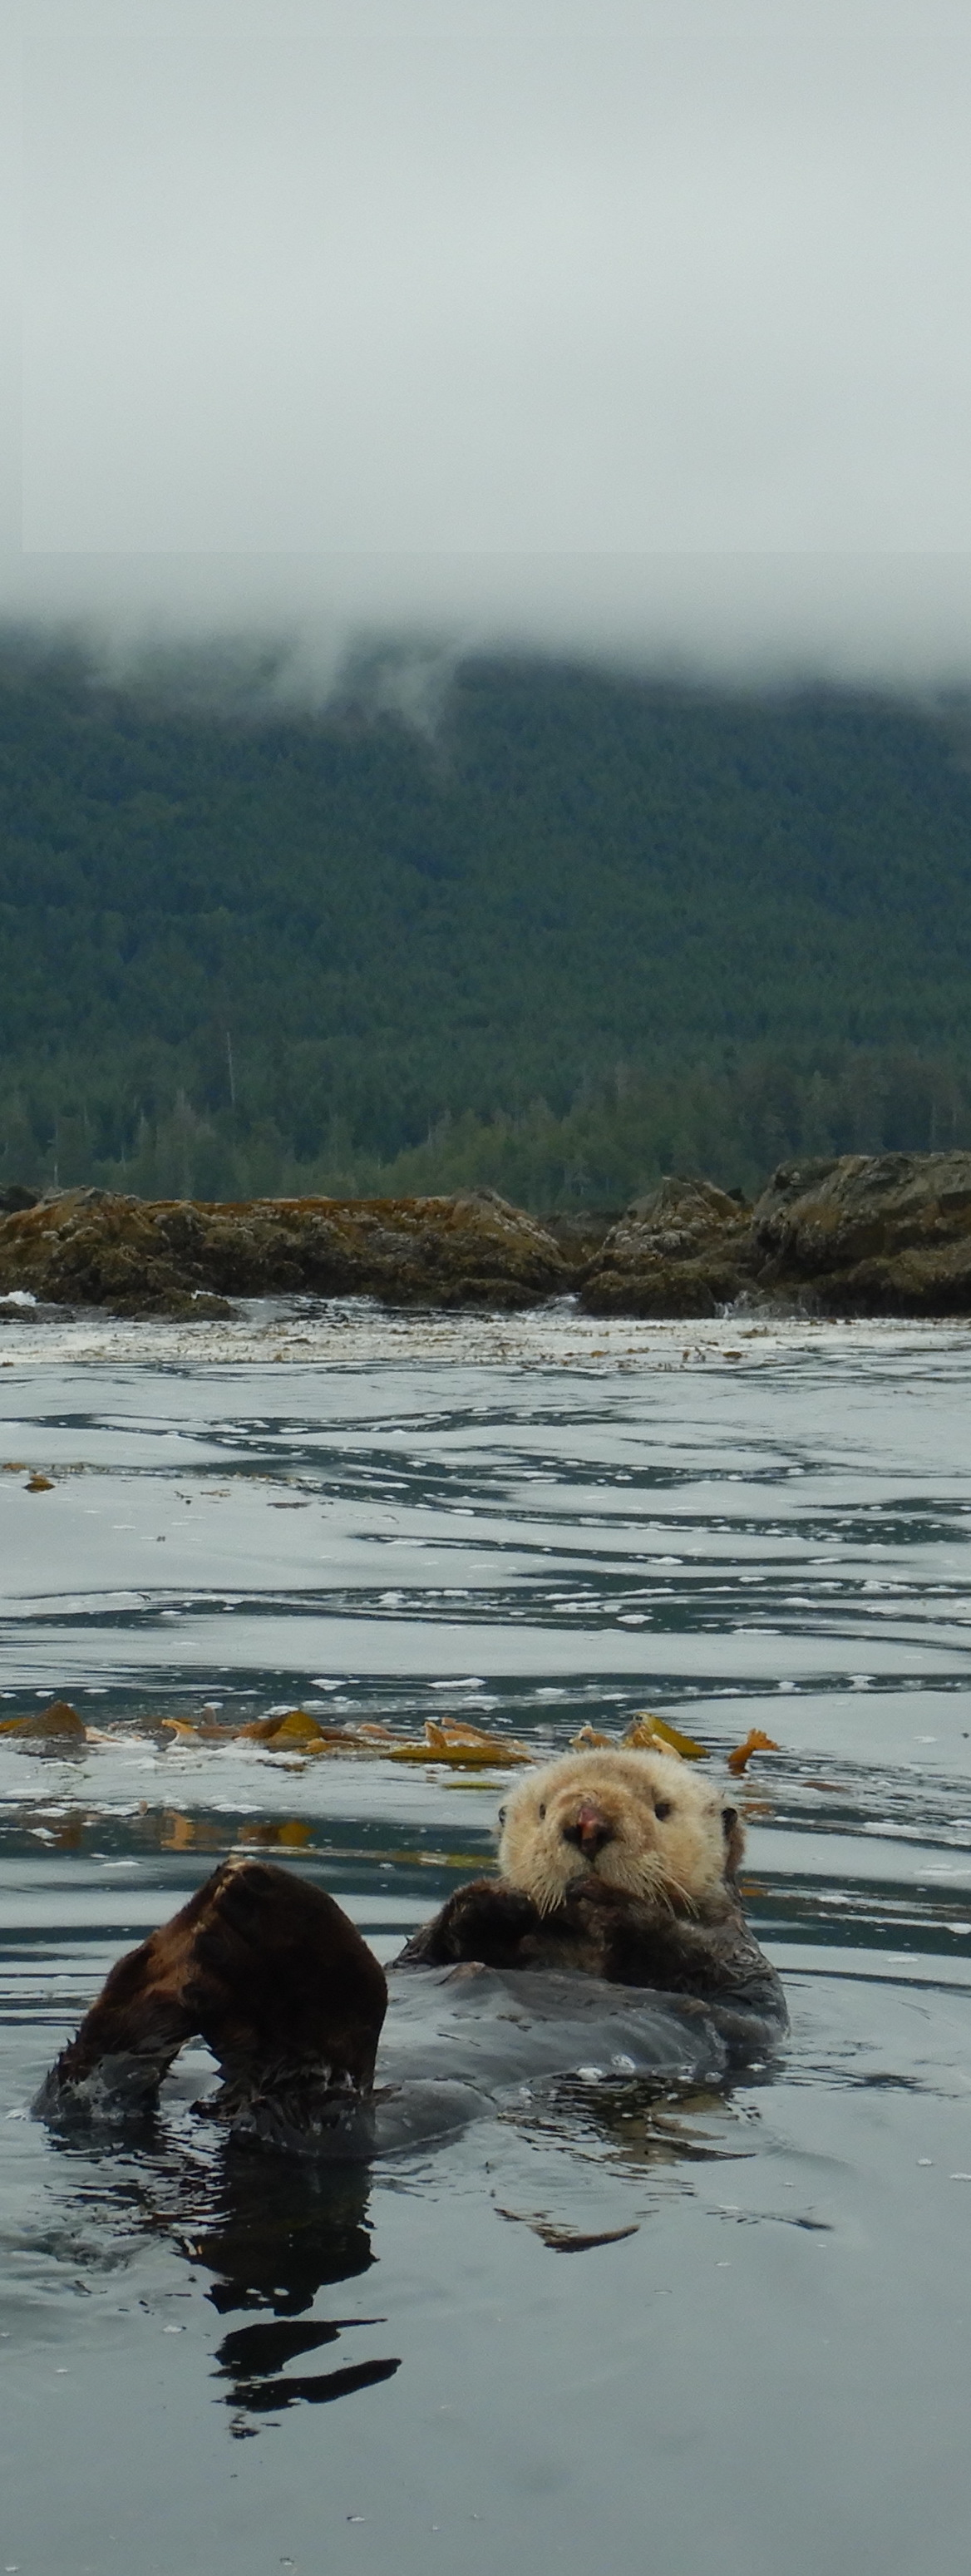
\includegraphics[%
width=1.0%
\paperwidth, keepaspectratio]{\_extensions/titlepage/images/otter-bar.jpeg}
};

% This section has the text and is theme specific
% Simple title

\newcommand{\titlelocationleft}{0.2\paperwidth}
\newcommand{\titlelocationbottom}{0.8\paperheight}
\newcommand{\titlealign}{left}

% Title
\begin{scope}
{%
\fontsize{100}{120.0} \coverpagetitlefont
\node[anchor=north west, align=left, rotate=45] (Title1) at %
($(current page.south west)+(\titlelocationleft,\titlelocationbottom)$)  [text width = 0.7000000000000001\paperwidth]  {
{A Sample Title - The SocioEconomic Aspects of Stock Assessments}};
}
\end{scope}
% Simple author

\newcommand{\authorlocationleft}{0.8\paperwidth}
\newcommand{\authorlocationbottom}{0.25\paperheight}
\newcommand{\authoralign}{right}

% Title
\begin{scope}
{%
\fontsize{30}{36.0} \coverpageauthorfont
\node[anchor=south east, align=right, rotate=0] (Author1) at %
($(current page.south west)+(\authorlocationleft,\authorlocationbottom)$)  [text width = 0.7000000000000001\paperwidth]  {
{Jane Doe\\Eva Nováková\\Matti Meikäläinen\\Ashok Kumar}};

}
\end{scope}

\end{tikzpicture}
\clearpage
\restoregeometry
% Use the file
% This is a combination of Pandoc templating and LaTeX
% Pandoc templating https://pandoc.org/MANUAL.html#templates
% See the README for help

% Get the theme commands
%Specify the titlepage alignments

%Page
\newcommand{\titlepagepagealign}{
\ifthenelse{\equal{left}{right}}{\raggedleft}{}
\ifthenelse{\equal{left}{center}}{\centering}{}
\ifthenelse{\equal{left}{left}}{\raggedright}{}
}

%% Titles
\newcommand{\titlepagetitlealign}{
\ifthenelse{\equal{}{right}}{\raggedleft}{}
\ifthenelse{\equal{}{center}}{\centering}{}
\ifthenelse{\equal{}{left}}{\raggedright}{}
\ifthenelse{\equal{}{spread}}{\makebox[\linewidth][s]}{}
}


%Author
\newcommand{\titlepageauthoralign}{
\ifthenelse{\equal{center}{right}}{\raggedleft}{}
\ifthenelse{\equal{center}{center}}{\centering}{}
\ifthenelse{\equal{center}{left}}{\raggedright}{}
\ifthenelse{\equal{center}{spread}}{\makebox[\linewidth][s]}{}
}

%Affiliation
\newcommand{\titlepageaffiliationalign}{
\ifthenelse{\equal{}{right}}{\raggedleft}{}
\ifthenelse{\equal{}{center}}{\centering}{}
\ifthenelse{\equal{}{left}}{\raggedright}{}
\ifthenelse{\equal{}{spread}}{\makebox[\linewidth][s]}{}
}


%Footer
\newcommand{\titlepagefooteralign}{
\ifthenelse{\equal{}{right}}{\raggedleft}{}
\ifthenelse{\equal{}{center}}{\centering}{}
\ifthenelse{\equal{}{left}}{\raggedright}{}
\ifthenelse{\equal{}{spread}}{\makebox[\linewidth][s]}{}
}

%Header
\newcommand{\titlepageheaderalign}{
\ifthenelse{\equal{}{right}}{\raggedleft}{}
\ifthenelse{\equal{}{center}}{\centering}{}
\ifthenelse{\equal{}{left}}{\raggedright}{}
\ifthenelse{\equal{}{spread}}{\makebox[\linewidth][s]}{}
}

%Logo
\newcommand{\titlepagelogoalign}{
\ifthenelse{\equal{}{right}}{\raggedleft}{}
\ifthenelse{\equal{}{center}}{\centering}{}
\ifthenelse{\equal{}{left}}{\raggedright}{}
}
% This file defines the author block and affiliation block
% based on the author and affiliation theme
% none, plain, colorbox, doublelined

\newcommand{\emptytitleblock}{}

\newcommand{\plaintitleblock}{
% Title and subtitle

{largebfseries\nohyphens{A Sample Title - The SocioEconomic Aspects of
Stock Assessments}}\\[1\baselineskip]

{largetextit{with non-English diacritics in the author names. see
documentation.}}\\}

\newcommand{\colorboxtitleblock}{
\setlength{\fboxrule}{4pt}
\fcolorbox{black}{cyan}{
	\parbox[t]{0.93\minipagewidth}{ % Outer full width box
		\parbox[t]{0.91\minipagewidth}{ % Inner box for inner right text margin
			\raggedright % Right align the text
			
			\vspace{0.7cm} % Space between the start of the title and the top of the grey box
			
			{largebfseries\nohyphens{A Sample Title - The SocioEconomic Aspects of
Stock Assessments}}\\
			
			{largetextit\nohyphens{with non-English diacritics in the author names.
see documentation.}}\\
			
			\vspace{0.7cm} % Space between the end of the title and the bottom of the grey box
		}
	}
}
}

\newcommand{\doublelinedtitleblock}{
\rule{\textwidth}{0.4pt} % Thin horizontal rule

\vspace{0.1\textheight} % Whitespace between the top rules and title

% Title and subtitle
{largebfseries\nohyphens{A Sample Title - The SocioEconomic Aspects of
Stock Assessments}}\\[1\baselineskip]
{{with non-English diacritics in the author names. see
documentation.}}\\

\vspace{0.025\textheight} 

\rule{0.3\textwidth}{0.4pt} % Short horizontal rule under the title
}

\newcommand{\titleandsubtitle}{
% Title and subtitle
{%

{\large \bfseries \nohyphens{A Sample Title - The SocioEconomic Aspects
of Stock Assessments}}%
}%

\vspace{\betweentitlesubtitle}
{%

{\large \textit \nohyphens{with non-English diacritics in the author
names. see documentation.}}%
}%
}


\newcommand{\titlepagetitleblock}{
\titleandsubtitle
}



\ifthenelse{\equal{}{none}}
{% True case
\newcommand{\coverpagetitleblock}{\emptytitleblock}
}{}
\ifthenelse{\equal{}{plain}}
{% True case
\newcommand{\coverpagetitleblock}{\plaintitleblock}
}{}
\ifthenelse{\equal{}{colorbox}}
{% True case
\newcommand{\coverpagetitleblock}{\colorboxtitleblock}
}{}

% This file defines the author block and affiliation block
% based on the author and affiliation theme
% none, plain, plain-with-and, plain-newline, plain-superscript, superscript, superscript-with-and, two-column

\newcommand{\authorstyle}{%

\large %
}
\newcommand{\affiliationstyle}{%

%
}

\newcommand{\emptyauthorblock}{}

\newcommand{\plainauthorblock}{
{\authorstyle
%
{Jane Doe}%
, %
%
{Eva Nováková}%
, %
%
{Matti Meikäläinen}%
, %
%
{Ashok Kumar}%

}
}

\newcommand{\plainauthornewlineblock}{
{\authorstyle
%
{Jane Doe}%
\\%
%
{Eva Nováková}%
\\%
%
{Matti Meikäläinen}%
\\%
%
{Ashok Kumar}%

}
}

\newcommand{\plainwithandauthorblock}{
{\authorstyle
%
%
{Jane Doe}%
, %
%
{Eva Nováková}%
, %
%
{Matti Meikäläinen}%
%
%
{ and Ashok Kumar}%
%

}
}

\newcommand{\plainsuperscriptauthorblock}{
{\authorstyle
%
{Jane Doe}%
%
{\textsuperscript{1}}{\textsuperscript{,}}%
%
{\textsuperscript{2}}%
%
 %
%
{Eva Nováková}%
%
{\textsuperscript{3}}%
%
 %
%
{Matti Meikäläinen}%
%
{\textsuperscript{4}}%
%
\textsuperscript{,}%
{\textsuperscript{*}}%
%
 %
%
{Ashok Kumar}%
%
{\textsuperscript{2}}{\textsuperscript{,}}%
%
{\textsuperscript{5}}%
%
%
}
}

\newcommand{\superscriptauthorblock}{
{\authorstyle
%
{Jane Doe}%
%
{\textsuperscript{1}}{\textsuperscript{,}}%
%
{\textsuperscript{2}}%
%
, %
%
{Eva Nováková}%
%
{\textsuperscript{3}}%
%
, %
%
{Matti Meikäläinen}%
%
{\textsuperscript{4}}%
%
\textsuperscript{,}%
{\textsuperscript{*}}%
%
, %
%
{Ashok Kumar}%
%
{\textsuperscript{2}}{\textsuperscript{,}}%
%
{\textsuperscript{5}}%
%
%
}
}

\newcommand{\superscriptwithandauthorblock}{
{\authorstyle
%
%
{Jane Doe}%
%
{\textsuperscript{1}}\textsuperscript{,}%
%
{\textsuperscript{2}}%
%
, %
%
{Eva Nováková}%
%
{\textsuperscript{3}}%
%
, %
%
{Matti Meikäläinen}%
%
{\textsuperscript{4}}%
%
\textsuperscript{,}%
{\textsuperscript{*}}%
%
%
%
{ and Ashok Kumar}%
%
{\textsuperscript{2}}\textsuperscript{,}%
%
{\textsuperscript{5}}%
%
%

}
}

\newcommand{\authoraddressblock}{
{\authorstyle
%
{Jane Doe}%
%
%
%
%
;~%
%
%
%
%
%

\\%
%
{Eva Nováková}%
%
%
%
%
%

\\%
%
{Matti Meikäläinen}%
%
%
%
%
%
~matti@jy.fi
\\%
%
{Ashok Kumar}%
%
%
%
%
;~%
%
%
%
%
%

%
}
}

\newcommand{\twocolumnauthorblock}{
\begin{minipage}{0.4\textwidth}
\begin{flushleft}
{\authorstyle
%
{Jane Doe}%
\\ %
%
{Eva Nováková}%
\\ %
%
{Matti Meikäläinen}%
\\ %
%
{Ashok Kumar}%
%
}
\end{flushleft}
\end{minipage}
~
\begin{minipage}{0.4\textwidth}
\begin{flushright}
{\affiliationstyle
%
{Minnesota Department of Natural Resources}%

%
{Czech University of Life Sciences}%

%
{University of Kemijärvi}%

%
{University of Minnesota}%

}
\end{flushright}
\end{minipage}
}

\newcommand{\numberedlistaffiliationblock}{
\hangindent=1em
\hangafter=1
{\affiliationstyle
%
{1}.~{Minnesota Department of Natural Resources}%
%
%
, %
{500 Lafayette Road Saint Paul, MN 55155}%
%
\par\hangindent=1em\hangafter=1%
%
{2}.~{University of Minnesota}%
%
, %
{Department of Mathematics}%
%
%
\par\hangindent=1em\hangafter=1%
%
{3}.~{Czech University of Life Sciences}%
%
%
, %
{Družstevní 666, Vikýřovice, Czechia}%
%
\par\hangindent=1em\hangafter=1%
%
{4}.~{University of Kemijärvi}%
%
, %
{Department of Biological and Environmental Science}%
%
%
, %
{Kylmäniementie 79, 98120, KEMIJÄRVI, Finland}%
%
\par\hangindent=1em\hangafter=1%
%
{5}.~{HØnefoss Institute}%
%
%
, %
{R Tradição 35, Portugal 2950-726}%
%

}
}

\newcommand{\numberedlistwithcorraffiliationblock}{
\hangindent=1em
\hangafter=1
{\affiliationstyle
%
{1}.~{Minnesota Department of Natural Resources}%
%
%
, %
{500 Lafayette Road Saint Paul, MN 55155}%
%
\par\hangindent=1em\hangafter=1%
%
{2}.~{University of Minnesota}%
%
, %
{Department of Mathematics}%
%
%
\par\hangindent=1em\hangafter=1%
%
{3}.~{Czech University of Life Sciences}%
%
%
, %
{Družstevní 666, Vikýřovice, Czechia}%
%
\par\hangindent=1em\hangafter=1%
%
{4}.~{University of Kemijärvi}%
%
, %
{Department of Biological and Environmental Science}%
%
%
, %
{Kylmäniementie 79, 98120, KEMIJÄRVI, Finland}%
%
\par\hangindent=1em\hangafter=1%
%
{5}.~{HØnefoss Institute}%
%
%
, %
{R Tradição 35, Portugal 2950-726}%
%


\vspace{1\baselineskip} 
* \textit{Correspondence:}~Matti Meikäläinen~matti@jy.fi
}
}


\ifthenelse{\equal{superscript-with-and}{none}}
{% True case
\newcommand{\titlepageauthorblock}{\emptyauthorblock}
}{}
\ifthenelse{\equal{}{none}}
{% True case
\newcommand{\coverpageauthorblock}{\emptyauthorblock}
}{}
\ifthenelse{\equal{superscript-with-and}{plain}}
{% True case
\newcommand{\titlepageauthorblock}{\plainauthorblock}
}{}
\ifthenelse{\equal{}{plain}}
{% True case
\newcommand{\coverpageauthorblock}{\plainauthorblock}
}{}
\ifthenelse{\equal{superscript-with-and}{plain-newline}}
{% True case
\newcommand{\titlepageauthorblock}{\plainauthornewlineblock}
}{}
\ifthenelse{\equal{}{plain-newline}}
{% True case
\newcommand{\coverpageauthorblock}{\plainauthornewlineblock}
}{}
\ifthenelse{\equal{superscript-with-and}{plain-with-and}}
{% True case
\newcommand{\titlepageauthorblock}{\plainwithandauthorblock}
}{}
\ifthenelse{\equal{}{plain-with-and}}
{% True case
\newcommand{\coverpageauthorblock}{\plainwithandauthorblock}
}{}
\ifthenelse{\equal{superscript-with-and}{plain-superscript}}
{% True case
\newcommand{\titlepageauthorblock}{\plainsuperscriptauthorblock}
}{}
\ifthenelse{\equal{superscript-with-and}{superscript}}
{% True case
\newcommand{\titlepageauthorblock}{\superscriptauthorblock}
}{}
\ifthenelse{\equal{superscript-with-and}{superscript-with-and}}
{% True case
\newcommand{\titlepageauthorblock}{\superscriptwithandauthorblock}
}{}
\ifthenelse{\equal{superscript-with-and}{two-column}}
{% True case
\newcommand{\titlepageauthorblock}{\twocolumnauthorblock}
}{}
\ifthenelse{\equal{}{two-column}}
{% True case
\newcommand{\coverpageauthorblock}{\twocolumnauthorblock}
}{}

\ifthenelse{\equal{numbered-list-with-correspondence}{none}}
{% True case
\newcommand{\titlepageaffiliationblock}{\emptyauthorblock}
}{}
\ifthenelse{\equal{numbered-list-with-correspondence}{numbered-list}}
{% True case
\newcommand{\titlepageaffiliationblock}{\numberedlistaffiliationblock}
}{}
\ifthenelse{\equal{numbered-list-with-correspondence}{numbered-list-with-correspondence}}
{% True case
\newcommand{\titlepageaffiliationblock}{\numberedlistwithcorraffiliationblock}
}{}


%set up blocks so user can specify order
\newcommand{\titleblock}{
\newlength{\betweentitlesubtitle}
\setlength{\betweentitlesubtitle}{1\baselineskip}
{\titlepagetitlealign
\titlepagetitlefont
{\titlepagetitleblock}
}
\newlength{\aftertitle}
\setlength{\aftertitle}{4\baselineskip}

\vspace{\aftertitle}
}

\newcommand{\authorblock}{
% Authors	
{\titlepageauthoralign
\titlepageauthorfont
{\titlepageauthorblock}
}
\newlength{\afterauthor}
\setlength{\afterauthor}{2\baselineskip}

\vspace{\afterauthor}
}

\newcommand{\affiliationblock}{
%%%%%% Affiliations
{\titlepageaffiliationalign
\titlepageaffiliationfont
\titlepageaffiliationblock
}
\newlength{\afteraffiliation}
\setlength{\afteraffiliation}{0pt}

\vspace{\afteraffiliation}
}

\newcommand{\logoblock}{
{\titlepagelogoalign

\includegraphics[width=0.25\textheight]{img/logo.png}
}
\newlength{\afterlogo}
\setlength{\afterlogo}{0.1\textheight}

\vspace{\afterlogo}
}

\newcommand{\footerblock}{
{\titlepagefooteralign
\titlepagefooterfont
{\noindent University Technical Series\\
Open Source Publication for All\\
Amtmandens Allé 15\\
6950 Rindum Ringkøbing-Skjern\\
DENMARK\\
December 2025}\\
}
\newlength{\afterfooter}
\setlength{\afterfooter}{0pt}

\vspace{\afterfooter}
}

\newcommand{\headerblock}{
{\titlepageheaderalign
\titlepageheaderfont
{\noindent The Publisher}\\
}
\newlength{\afterheader}
\setlength{\afterheader}{0pt}

\vspace{\afterheader}
}



% background image

\thispagestyle{empty} % no page numbers on titlepages
\titlepagefont

\newlength{\A}
\setlength{\A}{1pt}
\newlength{\B}
\setlength{\B}{\ifdim\A > 0pt 0.05\textheight\else 0pt\fi}
\newlength{\minipagewidth}
\ifthenelse{\equal{left}{left} \OR \equal{left}{right} }
{% True case
\setlength{\minipagewidth}{\textwidth - \A - \B - 0.1\textwidth}
}{
\setlength{\minipagewidth}{\textwidth - 2\A - 2\B - 0.1\textwidth}
}
\ifthenelse{\equal{left}{left} \OR \equal{left}{leftright}}
{% True case
\raggedleft % needed for the minipage to work
\rule{\A}{\textheight} % Vertical line
\hspace{\B} % Whitespace between the vertical line and title page text
}{%
% else it is right only and width is not 0
\raggedright}
% [position of box][box height][inner position]{width}
% [s] means stretch out vertically; assuming there is a vfill
\begin{minipage}[b][\textheight][s]{\minipagewidth}
\titlepagepagealign
\titleblock
\authorblock
\affiliationblock
\vfill
\logoblock
\footerblock
\end{minipage}

\ifthenelse{\equal{left}{right} \OR \equal{left}{leftright} }%
{% True case
\hspace{\B}
\rule{\A}{\textheight}
}{}
\end{titlepage}
\setcounter{page}{1}
\end{frontmatter}
\ifdefined\Shaded\renewenvironment{Shaded}{\begin{tcolorbox}[frame hidden, boxrule=0pt, enhanced, borderline west={3pt}{0pt}{shadecolor}, interior hidden, breakable, sharp corners]}{\end{tcolorbox}}\fi

\renewcommand*\contentsname{Table of contents}
{
\setcounter{tocdepth}{2}
\tableofcontents
}
\listoffigures
\listoftables
\mainmatter
\hypertarget{usage-notes}{%
\chapter{Usage notes}\label{usage-notes}}

\begin{verbatim}
    titlepage-theme: 
      elements: ["\\titleblock", "\\authorblock", "\\affiliationblock", "\\logoblock", "\\vfill", "\\footerblock"]
      page-html-color: "c4c4c4"
      page-text-align: left
      page-fontfamily: "Palatino"
      title-style: "plain"
      title-fontfamily: "Palatino"
      title-fontstyle: "\\Huge\\bfseries"
      title-align: left
      title-space-after: 1in
      subtitle-fontstyle: "\\large"
      author-style: "superscript"
      author-fontfamily: "Palatino"
      author-fontstyle: "\\large"
      author-align: left
      author-space-after: 1in
      affiliation-style: "numberedlist"
      affiliation-fontfamily: "Palatino"
      affiliation-fontstyle: "\\large"
      affiliation-align: left
      affiliation-space-after: 1in
      footer-style: "plain"
      footer-fontfamily: "Palatino"
      footer-fontstyle: "\\large"
      footer-align: left
      footer-space-after: 1in
      header-style: "plain"
      header-fontfamily: "Palatino"
      header-fontstyle: "\\large"
      header-align: left
      header-space-after: 1in
      logo-size: 0.25
      logo-space-after: 1in
      bg-image-size: 0.25
      bg-image-location: "URCorner"
      vrule-width: 20pt
      vrule-color: "blue"
      vrule-space-after: 10pt
\end{verbatim}

\hypertarget{yaml-additions-for-themes}{%
\section{YAML additions for themes}\label{yaml-additions-for-themes}}

Some themes need some additional YAML information to work.

\hypertarget{bg-image}{%
\subsection{\texorpdfstring{\texttt{bg-image}}{bg-image}}\label{bg-image}}

Needs info on the titlepage geometry so the title doesn't overlap the
background image. Also you need to supply the background image and where
to put it (UL, upperleft; UR, upperright; BL, bottomleft; BR,
bottomright). Note, there are placeholders in the extension, but when
you put your own image in, you'll need to add the YAML information.

\begin{verbatim}
format: 
  titlepage-pdf:
    titlepage: bg-image
    titlepage-geometry: 
     - top=3in
     - bottom=1in
     - right=1in
     - left=1in
    titlepage-image: "img/corner-bg.png"
    titlepage-image-location: "UL"
    titlepage-image-size: 0.5
\end{verbatim}

\hypertarget{great-wave}{%
\subsection{\texorpdfstring{\texttt{great-wave}}{great-wave}}\label{great-wave}}

Great wave cover page theme creates a cover page with a background image
that fills the width of the page at the bottom with a color above. You
need to specify the image and the upper color (unless you want to use
the default Great Wave off Kanagawa image).

\begin{verbatim}
coverpage-image: "img/TheGreatWaveoffKanagawa.jpeg"
coverpage-color: "F6D5A8"
\end{verbatim}

\hypertarget{document-classes}{%
\section{Document classes}\label{document-classes}}

The document class changes the look of your document. For the book
document classes, you will need to pass in

\begin{verbatim}
number-sections: true
\end{verbatim}

in your YAML because Quarto sets \texttt{number-sections:\ false} by
default and that will mess up all your equation, figure and table
numbers. It simple will not number them correctly at all.

For book document classes (like \texttt{scrbook}), if you want chapters
to be allowed to start on even or odd pages and the left and right
margins on even and odd pages to be the same, use

\begin{verbatim}
classoption: ["oneside", "open=any"]
\end{verbatim}

\hypertarget{static-versus-dynamic-themes}{%
\section{Static versus dynamic
themes}\label{static-versus-dynamic-themes}}

\texttt{vline-static}, \texttt{thesis-static},
\texttt{multi-purpose-static}, \texttt{classic-lined-static} and
\texttt{academic-static} use a title page that is defined in the
\texttt{\_extensions/titlepage} folder. You will need to edit the
\texttt{\_xyz-static\_titlepage.tex} file.

The other themes use the YAML for the title page info and you do not
need to edit the \texttt{...-titlepage.tex} files unless you want to
customize the pages.

\hypertarget{introduction}{%
\chapter{Introduction}\label{introduction}}

Lorem ipsum dolor sit amet, consectetur adipiscing elit. Proin eu tempor
velit. Fusce accumsan ultrices fringilla. Praesent sed odio mi. Mauris
non ligula turpis. Duis posuere lacus nec diam interdum dictum suscipit
magna molestie. Vestibulum nibh dolor, interdum eget rhoncus ut, sodales
eget justo. Morbi blandit lorem sit amet nulla egestas aliquam. Nunc
pharetra est at nibh ullamcorper in commodo erat dignissim. Cras et
suscipit enim.

Lorem ipsum dolor sit amet, consectetur adipiscing elit. Phasellus neque
ex, vehicula dictum risus fermentum, feugiat faucibus neque. Etiam purus
quam, lacinia vel porta in, malesuada ac nisl. Vestibulum ante ipsum
primis in faucibus orci luctus et ultrices posuere cubilia curae; Sed
bibendum placerat tellus, ac finibus lectus euismod eget.

Nulla mattis diam vitae bibendum consequat. Etiam vitae eros tristique,
porta sapien a, aliquet mauris. Praesent ultricies mi nulla, et
dignissim nulla mattis at. Fusce rhoncus leo quis odio euismod,
hendrerit facilisis risus tincidunt. Aenean at lectus justo. Cras
fringilla lacus nisl, ac convallis odio tincidunt vel. Integer vel
egestas nisi. Curabitur vitae imperdiet justo.

\begin{quote}
Lorem ipsum dolor sit amet, consectetur adipiscing elit, sed do eiusmod
tempor incididunt ut labore et dolore magna aliqua. Ut enim ad minim
veniam, quis nostrud exercitation ullamco laboris nisi ut aliquip ex ea
commodo consequat.\\
\end{quote}

\hypertarget{supporting-theory}{%
\section{Supporting theory}\label{supporting-theory}}

Let \(X_1, X_2, \ldots, X_n\) be a sequence of independent and
identically distributed random variables with \(\text{E}[X_i] = \mu\)
and \(\text{Var}[X_i] = \sigma^2 < \infty\), and let

\begin{equation}\protect\hypertarget{eq-clt}{}{
S_n = \frac{X_1 + X_2 + \cdots + X_n}{n}
      = \frac{1}{n}\sum_{i}^{n} X_i
}\label{eq-clt}\end{equation}

denote their mean. Then as \(n\) approaches infinity, the random
variables \(\sqrt{n}(S_n - \mu)\) converge in distribution to a normal
\(\mathcal{N}(0, \sigma^2)\). Thus concludes the explanation about
Equation~\ref{eq-clt}.

\hypertarget{materials-and-methods}{%
\chapter{Materials and Methods}\label{materials-and-methods}}

Lorem ipsum dolor sit amet, consectetur adipiscing elit. Phasellus neque
ex, vehicula dictum risus fermentum, feugiat faucibus neque. Etiam purus
quam, lacinia vel porta in, malesuada ac nisl. Vestibulum ante ipsum
primis in faucibus orci luctus et ultrices posuere cubilia curae; Sed
bibendum placerat tellus, ac finibus lectus euismod eget.

\hypertarget{study-area}{%
\section{Study area}\label{study-area}}

Lorem ipsum dolor sit amet, consectetur adipiscing elit. Phasellus neque
ex, vehicula dictum risus fermentum, feugiat faucibus neque. Etiam purus
quam, lacinia vel porta in, malesuada ac nisl. Vestibulum ante ipsum
primis in faucibus orci luctus et ultrices posuere cubilia curae; Sed
bibendum placerat tellus, ac finibus lectus euismod eget. Nulla mattis
diam vitae bibendum consequat.

\begin{figure}

{\centering 
\includegraphics{logo.png}

}

\caption{\label{fig-logo}the study area}

\end{figure}

See Figure~\ref{fig-logo} for a picture of the study area. Etiam vitae
eros tristique, porta sapien a, aliquet mauris. Praesent ultricies mi
nulla, et dignissim nulla mattis at. Fusce rhoncus leo quis odio
euismod, hendrerit facilisis risus tincidunt. Aenean at lectus justo.
Cras fringilla lacus nisl, ac convallis odio tincidunt vel. Integer vel
egestas nisi. Curabitur vitae imperdiet justo.

Curabitur efficitur in risus quis egestas. Suspendisse porta interdum
leo ac ultricies. Pellentesque bibendum, felis vitae fermentum eleifend,
nunc nunc fermentum nisi, ac maximus felis lacus lobortis risus.
Suspendisse potenti. Nunc vitae consequat elit. Fusce id ligula sed
lectus condimentum laoreet. Vestibulum faucibus commodo suscipit. Nulla
tempor tellus vel massa efficitur euismod. Duis nec commodo mauris, sit
amet tincidunt elit. Cras mollis non ante sed venenatis. In ultricies
ante accumsan lectus rhoncus, vel pharetra sem convallis.

\hypertarget{results}{%
\chapter{Results}\label{results}}

See Table~\ref{tbl-numbers} for the table of results. Phasellus quis
orci nec erat suscipit imperdiet. Aenean pulvinar enim ut ante
convallis, vel sollicitudin purus malesuada. Sed sed ullamcorper urna.
Morbi sed lobortis neque, sit amet hendrerit magna. Donec ultricies
pretium lorem, eget sagittis metus posuere et. Aenean ex purus, aliquam
sit amet tellus ut, pellentesque porttitor orci. Integer quis mi
pharetra, bibendum neque nec, viverra nulla. Cras quis magna in erat
facilisis consequat. Vivamus sed lectus iaculis, euismod ligula eu,
fermentum sem.

\hypertarget{tbl-numbers}{}
\begin{longtable}[]{@{}lr@{}}
\caption{\label{tbl-numbers}Table of numbers.}\tabularnewline
\toprule()
Thing & Value \\
\midrule()
\endfirsthead
\toprule()
Thing & Value \\
\midrule()
\endhead
A 42 & 18 \\
B 15 & 18 \\
C 34 & 17 \\
D 99 & 24 \\
\bottomrule()
\end{longtable}

\hypertarget{discussion}{%
\chapter{Discussion}\label{discussion}}

Lorem ipsum dolor sit amet, Table~\ref{tbl-numbers}, consectetur
adipiscing elit. Knuth (1984) and all things LaTeX. Phasellus neque ex,
vehicula dictum risus fermentum, feugiat faucibus neque. Etiam purus
quam, lacinia vel porta in, malesuada ac nisl. Vestibulum ante ipsum
primis in faucibus orci luctus et ultrices posuere cubilia curae; Sed
bibendum placerat tellus, ac finibus lectus euismod eget. Nulla mattis
diam vitae bibendum consequat. Etiam vitae eros tristique, porta sapien
a, aliquet mauris. Praesent ultricies mi nulla, et dignissim nulla
mattis at. Fusce rhoncus leo quis odio euismod, hendrerit facilisis
risus tincidunt. Aenean at lectus justo. Cras fringilla lacus nisl, ac
convallis odio tincidunt vel. Integer vel egestas nisi. Curabitur vitae
imperdiet justo.

Curabitur efficitur in risus quis egestas. Suspendisse porta interdum
leo ac ultricies. Pellentesque bibendum, felis vitae fermentum eleifend,
nunc nunc fermentum nisi, ac maximus felis lacus lobortis risus.
Suspendisse potenti. Nunc vitae consequat elit. Fusce id ligula sed
lectus condimentum laoreet. Vestibulum faucibus commodo suscipit. Nulla
tempor tellus vel massa efficitur euismod. Duis nec commodo mauris, sit
amet tincidunt elit. Cras mollis non ante sed venenatis. In ultricies
ante accumsan lectus rhoncus, vel pharetra sem convallis.

Phasellus quis orci nec erat suscipit imperdiet. Aenean pulvinar enim ut
ante convallis, vel sollicitudin purus malesuada. Sed sed ullamcorper
urna. Morbi sed lobortis neque, sit amet hendrerit magna. Donec
ultricies pretium lorem, eget sagittis metus posuere et. Aenean ex
purus, aliquam sit amet tellus ut, pellentesque porttitor orci. Integer
quis mi pharetra, bibendum neque nec, viverra nulla. Cras quis magna in
erat facilisis consequat. Vivamus sed lectus iaculis, euismod ligula eu,
fermentum sem.

Quisque congue, ligula et mattis vulputate, arcu risus facilisis mauris,
a feugiat mi mi et magna. Aliquam id malesuada neque. Sed dapibus justo
mauris, sed mattis nibh sodales sit amet. Donec nec faucibus magna.
Curabitur tincidunt porta egestas. In eleifend sed enim ac varius.
Vivamus tempus ultrices vehicula. Vestibulum iaculis eleifend mattis.
Quisque euismod dui et velit facilisis dapibus. Ut in mauris porttitor,
congue orci et, sodales turpis. Pellentesque porttitor volutpat sapien
vel pretium.

Aliquam ante diam, euismod in nisi sed, iaculis tincidunt lacus. Cras
pellentesque magna id enim pulvinar porta. Proin quis feugiat quam. Nunc
vitae ultricies nulla, a facilisis tortor. Aliquam semper mi et libero
tincidunt, nec iaculis erat pharetra. Duis ac pharetra purus. Nunc
condimentum ex massa, a vestibulum risus bibendum in. Suspendisse
suscipit, lectus pharetra vulputate fringilla, ligula sem condimentum
purus, eget dapibus diam libero vitae lorem. Nam blandit pulvinar augue,
non gravida risus rhoncus sed.

\hypertarget{conclusion}{%
\chapter{Conclusion}\label{conclusion}}

Lorem ipsum dolor sit amet, consectetur adipiscing elit. Phasellus neque
ex, vehicula dictum risus fermentum, feugiat faucibus neque. Etiam purus
quam, lacinia vel porta in, malesuada ac nisl. Vestibulum ante ipsum
primis in faucibus orci luctus et ultrices posuere cubilia curae; Sed
bibendum placerat tellus, ac finibus lectus euismod eget. Nulla mattis
diam vitae bibendum consequat. Etiam vitae eros tristique, porta sapien
a, aliquet mauris. Praesent ultricies mi nulla, et dignissim nulla
mattis at. Fusce rhoncus leo quis odio euismod, hendrerit facilisis
risus tincidunt. Aenean at lectus justo. Cras fringilla lacus nisl, ac
convallis odio tincidunt vel. Integer vel egestas nisi. Curabitur vitae
imperdiet justo.

Curabitur efficitur in risus quis egestas. Suspendisse porta interdum
leo ac ultricies. Pellentesque bibendum, felis vitae fermentum eleifend,
nunc nunc fermentum nisi, ac maximus felis lacus lobortis risus.
Suspendisse potenti. Nunc vitae consequat elit. Fusce id ligula sed
lectus condimentum laoreet. Vestibulum faucibus commodo suscipit. Nulla
tempor tellus vel massa efficitur euismod. Duis nec commodo mauris, sit
amet tincidunt elit. Cras mollis non ante sed venenatis. In ultricies
ante accumsan lectus rhoncus, vel pharetra sem convallis.

Phasellus quis orci nec erat suscipit imperdiet. Aenean pulvinar enim ut
ante convallis, vel sollicitudin purus malesuada. Sed sed ullamcorper
urna. Morbi sed lobortis neque, sit amet hendrerit magna. Donec
ultricies pretium lorem, eget sagittis metus posuere et. Aenean ex
purus, aliquam sit amet tellus ut, pellentesque porttitor orci. Integer
quis mi pharetra, bibendum neque nec, viverra nulla. Cras quis magna in
erat facilisis consequat. Vivamus sed lectus iaculis, euismod ligula eu,
fermentum sem.

Quisque congue, ligula et mattis vulputate, arcu risus facilisis mauris,
a feugiat mi mi et magna. Aliquam id malesuada neque. Sed dapibus justo
mauris, sed mattis nibh sodales sit amet. Donec nec faucibus magna.
Curabitur tincidunt porta egestas. In eleifend sed enim ac varius.
Vivamus tempus ultrices vehicula. Vestibulum iaculis eleifend mattis.
Quisque euismod dui et velit facilisis dapibus. Ut in mauris porttitor,
congue orci et, sodales turpis. Pellentesque porttitor volutpat sapien
vel pretium.

Aliquam ante diam, euismod in nisi sed, iaculis tincidunt lacus. Cras
pellentesque magna id enim pulvinar porta. Proin quis feugiat quam. Nunc
vitae ultricies nulla, a facilisis tortor. Aliquam semper mi et libero
tincidunt, nec iaculis erat pharetra. Duis ac pharetra purus. Nunc
condimentum ex massa, a vestibulum risus bibendum in. Suspendisse
suscipit, lectus pharetra vulputate fringilla, ligula sem condimentum
purus, eget dapibus diam libero vitae lorem. Nam blandit pulvinar augue,
non gravida risus rhoncus sed.

\hypertarget{author-contributions}{%
\chapter{Author Contributions}\label{author-contributions}}

Author1 designed the research. Author2 carried out all simulations,
analyzed the data. Author1 and Author2 wrote the article.

\hypertarget{acknowledgments}{%
\chapter{Acknowledgments}\label{acknowledgments}}

We thank G. Harrison, B. Harper, and J. Doe for their help.

\hypertarget{references}{%
\chapter{References}\label{references}}

\hypertarget{refs}{}
\begin{CSLReferences}{1}{0}
\leavevmode\vadjust pre{\hypertarget{ref-knuth84}{}}%
Knuth, Donald E. 1984. {``Literate Programming.''} \emph{Comput. J.} 27
(2): 97--111. \url{https://doi.org/10.1093/comjnl/27.2.97}.

\end{CSLReferences}


\backmatter

\end{document}
